\documentclass[sigconf, 10pt, nonacm]{acmart}
\usepackage[moderate]{savetrees}

\newcommand{\alek}[1]{\textcolor{red}{#1}}

\usepackage{booktabs} % For formal tables
\usepackage{appendix}


% Copyright
%\setcopyright{none}
%\setcopyright{acmcopyright}
%\setcopyright{acmlicensed}
\setcopyright{rightsretained}
%\setcopyright{usgov}
%\setcopyright{usgovmixed}
%\setcopyright{cagov}
%\setcopyright{cagovmixed}


% DOI
\acmDOI{10.475/123_4}

% ISBN
\acmISBN{123-4567-24-567/08/06}

%Conference
%% \acmConference[APOCS '20]{}{January 2020}{Salt Lake City, UT, USA}
%% \acmYear{2019}
%% \copyrightyear{2019}


\acmArticle{4}
\acmPrice{15.00}

\usepackage{mathtools}
\newcommand{\defeq}{\vcentcolon=}
\DeclarePairedDelimiter{\paren}{(}{)}

\usepackage{enumitem}
\usepackage{subcaption}

\usepackage{tikz,pgfplots}
\usepackage{etoolbox}
%% This makes the colors annoyingly bright, but at least they're easy to distinguish.
\pgfplotsset{
  every  tick/.style={red,}, minor x tick num=1,
  cycle list={teal,every mark/.append style={fill=teal!80!black},mark=*\\%
orange,every mark/.append style={fill=orange!80!black},mark=square*\\%
cyan!60!black,every mark/.append style={fill=cyan!80!black},mark=otimes*\\%
red!70!white,mark=star\\%
lime!80!black,every mark/.append style={fill=lime},mark=diamond*\\%
red,densely dashed,every mark/.append style={solid,fill=red!80!black},mark=*\\%
yellow!60!black,densely dashed,
every mark/.append style={solid,fill=yellow!80!black},mark=square*\\%
black,every mark/.append style={solid,fill=gray},mark=otimes*\\%
blue,densely dashed,mark=star,every mark/.append style=solid\\%
red,densely dashed,every mark/.append style={solid,fill=red!80!black},mark=diamond*\\%
}
}

%% Issues: One }; missing in bandwidth table by default
%% Same issue appears multiple times in sort table

\def \CILKserialbaseline {3932.2}
\def \CILKblocksize {64}
\def \CILKnumtrials {5}
\def \CILKinputsize {1073741824}
\def \CILKtable {
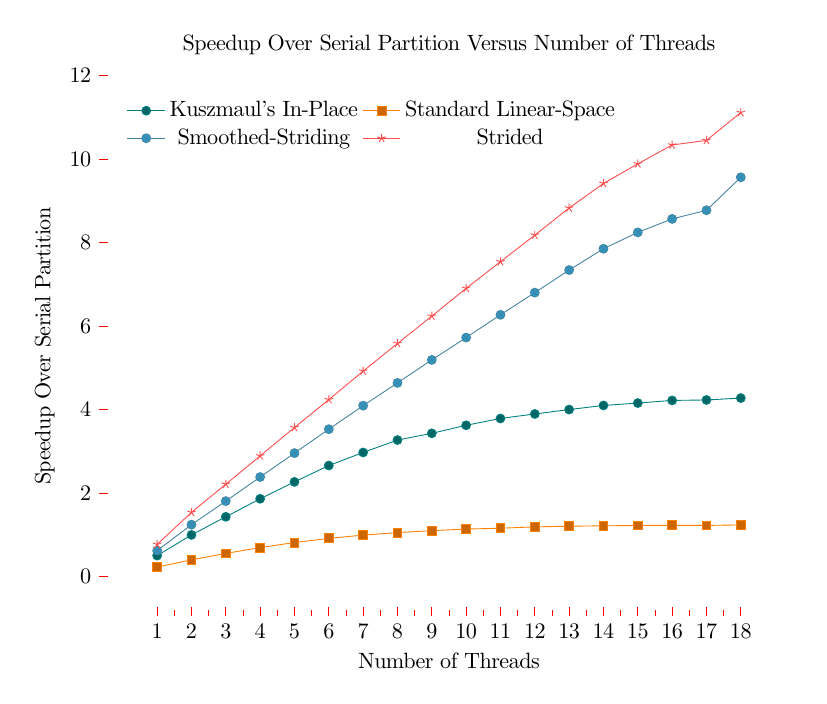
\begin{tikzpicture}[scale = .8]
\begin{axis}[
width = 5 in,
height = 4in,
title={Speedup Over Serial Partition Versus Number of Threads},
xtick pos=left,
ytick pos=left,
legend style={draw=none},
axis line style = { draw = none },
legend pos= north west,
xtick = data,
xlabel={Number of Threads},
ylabel={Speedup Over Serial Partition},
ymax = 12,
legend columns = 2,
scatter/classes=%
{a={mark=o,draw=blue}}]
%% In-Place
\addplot coordinates {( 1, 0.499048) ( 2, 0.995494) ( 3, 1.42948) ( 4, 1.86113) ( 5, 2.26614) ( 6, 2.65797) ( 7, 2.97174) ( 8, 3.26921) ( 9, 3.43004) ( 10, 3.62281) ( 11, 3.78679) ( 12, 3.89481) ( 13, 4.0002) ( 14, 4.0986) ( 15, 4.15578) ( 16, 4.2191) ( 17, 4.22999) ( 18, 4.27599) };
%% In-Place Prefix-Sum
% \addplot coordinates {( 1, 0.35092) ( 2, 0.636608) ( 3, 0.894292) ( 4, 1.11755) ( 5, 1.32674) ( 6, 1.5096) ( 7, 1.65121) ( 8, 1.77494) ( 9, 1.88432) ( 10, 1.97837) ( 11, 2.0581) ( 12, 2.11591) ( 13, 2.15699) ( 14, 2.18845) ( 15, 2.21159) ( 16, 2.21657) ( 17, 2.20736) ( 18, 2.21557) };
%% Out-of-Place
\addplot coordinates {( 1, 0.223968) ( 2, 0.398625) ( 3, 0.551717) ( 4, 0.691607) ( 5, 0.812203) ( 6, 0.912936) ( 7, 0.990429) ( 8, 1.05055) ( 9, 1.09777) ( 10, 1.13562) ( 11, 1.15517) ( 12, 1.18848) ( 13, 1.20383) ( 14, 1.21364) ( 15, 1.22103) ( 16, 1.22575) ( 17, 1.22285) ( 18, 1.23444) };
%% %% High-Span
%% \addplot coordinates {( 1, 0.796443) ( 2, 1.58021) ( 3, 2.21882) ( 4, 2.93667) ( 5, 3.32899) ( 6, 3.80217) ( 7, 4.3662) ( 8, 4.93375) ( 9, 5.09881) ( 10, 5.42822) ( 11, 5.75051) ( 12, 6.01806) ( 13, 6.37103) ( 14, 6.57999) ( 15, 6.72631) ( 16, 6.95718) ( 17, 7.06722) ( 18, 7.34442) };
%% Cache-Friendly
\addplot coordinates {( 1, 0.619888) ( 2, 1.24099) ( 3, 1.80558) ( 4, 2.38286) ( 5, 2.95654) ( 6, 3.52917) ( 7, 4.09348) ( 8, 4.63922) ( 9, 5.19034) ( 10, 5.72539) ( 11, 6.27145) ( 12, 6.80311) ( 13, 7.34442) ( 14, 7.85497) ( 15, 8.24706) ( 16, 8.57062) ( 17, 8.77723) ( 18, 9.5674) };
%% Strided
\addplot coordinates {( 1, 0.767408) ( 2, 1.5359) ( 3, 2.21084) ( 4, 2.89005) ( 5, 3.56954) ( 6, 4.2382) ( 7, 4.9214) ( 8, 5.58393) ( 9, 6.23961) ( 10, 6.90587) ( 11, 7.54451) ( 12, 8.18186) ( 13, 8.83243) ( 14, 9.4207) ( 15, 9.88984) ( 16, 10.3425) ( 17, 10.4524) ( 18, 11.1205) };
\legend{Kuszmaul's In-Place, Standard Linear-Space, Smoothed-Striding, Strided} %% Low-Space, Med-Space, High-Space, Smoothed-Striding, Strided 
\end{axis}
\end{tikzpicture}
}
\def \partitionbandwidthboundserialbaseline {3933.6}
\def \partitionbandwidthboundblocksize {64}
\def \partitionbandwidthboundnumtrials {5}
\def \partitionbandwidthboundinputsize {1073741824}
\def \partitionbandwidthboundtable {
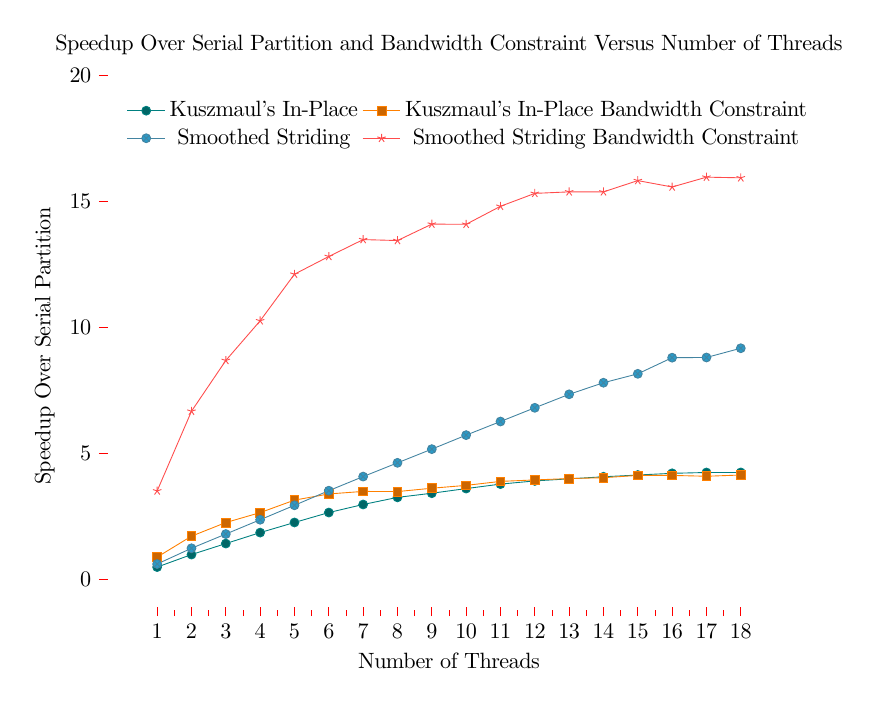
\begin{tikzpicture}[scale = .8]
\begin{axis}[
width = 5 in,
height = 4in,
title={Speedup Over Serial Partition and Bandwidth Constraint Versus Number of Threads},
xtick pos=left,
ytick pos=left,
legend style={draw=none},
axis line style = { draw = none },
legend pos= north west,
xtick = data,
xlabel={Number of Threads},
ylabel={Speedup Over Serial Partition},
ymax = 20,
legend columns = 2,
scatter/classes=%
{a={mark=o,draw=blue}}]
%% In-Place
\addplot coordinates {( 1, 0.499378) ( 2, 0.995949) ( 3, 1.4328) ( 4, 1.86816) ( 5, 2.26982) ( 6, 2.66432) ( 7, 2.98407) ( 8, 3.26602) ( 9, 3.43066) ( 10, 3.61544) ( 11, 3.79325) ( 12, 3.91949) ( 13, 4.00244) ( 14, 4.08389) ( 15, 4.15375) ( 16, 4.22151) ( 17, 4.25438) ( 18, 4.25622) };
%% Low-Space Bandwidth Bound
\addplot coordinates {(1, 0.894939)(2, 1.72634)(3, 2.26699)(4, 2.66131)(5, 3.15777)(6, 3.4024)(7, 3.50312)(8, 3.49686)(9, 3.62955)(10, 3.74294)(11, 3.90093)(12, 3.9593)(13, 4.0131)(14, 4.04714)(15, 4.13799)(16, 4.13782)(17, 4.10515)(18, 4.15355)};
%% high span
%% \addplot coordinates {( 1, 0.812828) ( 2, 1.61997) ( 3, 2.22137) ( 4, 2.95626) ( 5, 3.33582) ( 6, 3.80352) ( 7, 4.36001) ( 8, 5.10062) ( 9, 5.11521) ( 10, 5.44217) ( 11, 5.74752) ( 12, 6.07787) ( 13, 6.41278) ( 14, 6.63787) ( 15, 6.68752) ( 16, 6.79848) ( 17, 7.10549) ( 18, 7.26292) };
%% %% High-Span Bandwidth Bound
%% \addplot coordinates {(1, 1.75849)(2, 3.34185)(3, 4.35383)(4, 5.15739)(5, 5.9788)(6, 6.31621)(7, 6.76074)(8, 6.76348)(9, 6.99773)(10, 7.10173)(11, 7.39957)(12, 7.51437)(13, 7.7436)(14, 7.76191)(15, 7.89966)(16, 7.87403)(17, 7.94484)(18, 8.05483)}; %% cache friendly
\addplot coordinates {( 1, 0.62101) ( 2, 1.24639) ( 3, 1.81072) ( 4, 2.37852) ( 5, 2.95182) ( 6, 3.53233) ( 7, 4.09153) ( 8, 4.63759) ( 9, 5.18124) ( 10, 5.73746) ( 11, 6.27769) ( 12, 6.82206) ( 13, 7.35802) ( 14, 7.81717) ( 15, 8.17117) ( 16, 8.81183) ( 17, 8.81973) ( 18, 9.18636) };
%% Cache-Friendly Bandwidth Bound
\addplot coordinates {(1, 3.52223)(2, 6.68603)(3, 8.70095)(4, 10.276)(5, 12.1258)(6, 12.8292)(7, 13.4991)(8, 13.4622)(9, 14.1134)(10, 14.1066)(11, 14.8215)(12, 15.3338)(13, 15.3938)(14, 15.3942)(15, 15.8412)(16, 15.5877)(17, 15.9778)(18, 15.9519)};
\legend{Kuszmaul's In-Place, Kuszmaul's In-Place Bandwidth Constraint, Smoothed Striding, Smoothed Striding Bandwidth Constraint}
\end{axis}
\end{tikzpicture}
}

\def \CILKsortblocksize {64}
\def \CILKsortnumtrials {5}
\def \CILKsortmaxinputsize {1073741824}
\def \CILKsorttable {
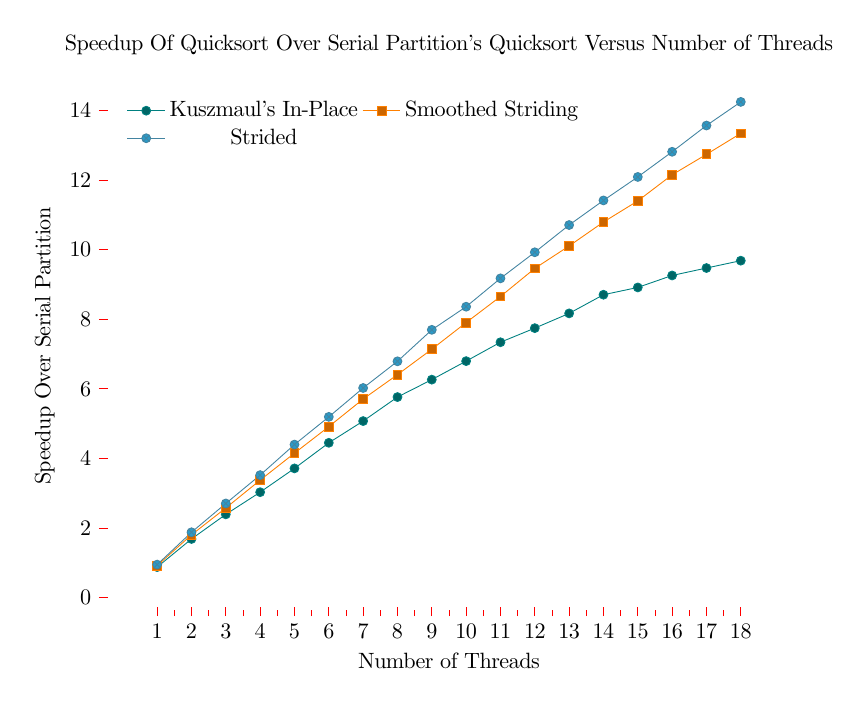
\begin{tikzpicture}[scale = .8]
\begin{axis}[
width = 5 in,
height = 4in,
title={Speedup Of Quicksort Over Serial Partition's Quicksort Versus Number of Threads},
xtick pos=left,
ytick pos=left,
legend style={draw=none},
axis line style = { draw = none },
legend pos= north west,
xtick = data,
xlabel={Number of Threads},
ylabel={Speedup Over Serial Partition},
ymax = 15,
legend columns = 2,
scatter/classes=%
{a={mark=o,draw=blue}}]
%% %% Low Space with log size 24
%% \addplot coordinates {( 1, 0.863202) ( 2, 1.63232) ( 3, 2.29705) ( 4, 2.96413) ( 5, 3.59298) ( 6, 4.1696) ( 7, 4.71085) ( 8, 5.2279) ( 9, 5.8474) ( 10, 6.4043) ( 11, 6.55736) ( 12, 7.21241) ( 13, 7.57064) ( 14, 7.99417) ( 15, 8.4679) ( 16, 8.93099) ( 17, 9.04881) ( 18, 9.60644) %% High-Span with log size 24
%% \addplot coordinates {( 1, 0.960106) ( 2, 1.88538) ( 3, 2.72075) ( 4, 3.47467) ( 5, 4.2576) ( 6, 5.08451) ( 7, 5.93339) ( 8, 6.47686) ( 9, 7.1822) ( 10, 7.57901) ( 11, 8.44704) ( 12, 8.64943) ( 13, 9.16979) ( 14, 9.04881) ( 15, 10.1464) ( 16, 9.61992) ( 17, 10.5199) ( 18, 9.38304) %% Cache Friendly with log size 24
%% \addplot coordinates {( 1, 0.900013) ( 2, 1.74752) ( 3, 2.46372) ( 4, 3.23233) ( 5, 3.90159) ( 6, 4.62508) ( 7, 5.46099) ( 8, 6.15157) ( 9, 6.85215) ( 10, 7.53736) ( 11, 8.11716) ( 12, 8.74872) ( 13, 9.70156) ( 14, 9.04881) ( 15, 11.0273) ( 16, 10.87) ( 17, 12.1829) ( 18, 12.2482) %% Strided with log size 24
%% \addplot coordinates {( 1, 0.95079) ( 2, 1.82955) ( 3, 2.63808) ( 4, 3.45716) ( 5, 4.20798) ( 6, 4.99199) ( 7, 5.78819) ( 8, 6.56364) ( 9, 7.37527) ( 10, 8.03162) ( 11, 8.89624) ( 12, 9.61992) ( 13, 9.7153) ( 14, 11.1167) ( 15, 10.9394) ( 16, 11.4891) ( 17, 13.1651) ( 18, 13.9695) };
%% %% Low Space with log size 26
%% \addplot coordinates {( 1, 0.861043) ( 2, 1.63325) ( 3, 2.3004) ( 4, 2.98343) ( 5, 3.63316) ( 6, 4.19898) ( 7, 4.82886) ( 8, 5.34581) ( 9, 5.89992) ( 10, 6.44372) ( 11, 6.94206) ( 12, 7.4672) ( 13, 7.60676) ( 14, 8.0564) ( 15, 8.64475) ( 16, 8.82709) ( 17, 8.76202) ( 18, 8.96831) %% High-Span with log size 26
%% \addplot coordinates {( 1, 0.955523) ( 2, 1.86586) ( 3, 2.6845) ( 4, 3.49224) ( 5, 4.27081) ( 6, 5.0929) ( 7, 5.83274) ( 8, 6.53586) ( 9, 7.29308) ( 10, 7.90003) ( 11, 8.63721) ( 12, 8.97915) ( 13, 9.7769) ( 14, 10.1893) ( 15, 10.5812) ( 16, 10.7887) ( 17, 10.7613) ( 18, 10.3418) %% Cache Friendly with log size 26
%% \addplot coordinates {( 1, 0.914609) ( 2, 1.73339) ( 3, 2.49178) ( 4, 3.22151) ( 5, 4.02384) ( 6, 4.70946) ( 7, 5.57239) ( 8, 6.13884) ( 9, 6.93881) ( 10, 7.59315) ( 11, 8.23047) ( 12, 8.91717) ( 13, 9.42939) ( 14, 10.1302) ( 15, 10.6801) ( 16, 10.8359) ( 17, 11.3883) ( 18, 11.3189) %% Strided with log size 26
%% \addplot coordinates {( 1, 0.946785) ( 2, 1.82922) ( 3, 2.64766) ( 4, 3.4262) ( 5, 4.2788) ( 6, 5.08245) ( 7, 5.95192) ( 8, 6.67986) ( 9, 7.44475) ( 10, 8.25563) ( 11, 8.94132) ( 12, 9.74164) ( 13, 10.4362) ( 14, 11.3621) ( 15, 11.4851) ( 16, 12.2071) ( 17, 12.6542) ( 18, 13.4993) };
%% %% Low Space with log size 28
%% \addplot coordinates {( 1, 0.862267) ( 2, 1.63941) ( 3, 2.34664) ( 4, 2.96157) ( 5, 3.64611) ( 6, 4.31258) ( 7, 4.88345) ( 8, 5.43042) ( 9, 5.87762) ( 10, 6.44029) ( 11, 7.00878) ( 12, 7.30452) ( 13, 7.83539) ( 14, 8.12956) ( 15, 8.50856) ( 16, 8.76302) ( 17, 8.98741) ( 18, 9.33821) %% High-Span with log size 28
%% \addplot coordinates {( 1, 0.939362) ( 2, 1.84744) ( 3, 2.6917) ( 4, 3.45716) ( 5, 4.29244) ( 6, 5.08279) ( 7, 5.79208) ( 8, 6.6353) ( 9, 7.2093) ( 10, 8.01682) ( 11, 8.74742) ( 12, 9.17326) ( 13, 9.7479) ( 14, 10.2979) ( 15, 11.0745) ( 16, 11.4344) ( 17, 11.4888) ( 18, 12.34) %% Cache Friendly with log size 28
%% \addplot coordinates {( 1, 0.908881) ( 2, 1.75263) ( 3, 2.51771) ( 4, 3.28228) ( 5, 4.01042) ( 6, 4.74982) ( 7, 5.54834) ( 8, 6.2393) ( 9, 6.98884) ( 10, 7.70125) ( 11, 8.41219) ( 12, 9.06778) ( 13, 9.67555) ( 14, 10.3505) ( 15, 11.0125) ( 16, 11.4744) ( 17, 12.1533) ( 18, 12.4095) %% Strided with log size 28
%% \addplot coordinates {( 1, 0.942529) ( 2, 1.82563) ( 3, 2.6044) ( 4, 3.46053) ( 5, 4.25683) ( 6, 5.12315) ( 7, 5.88602) ( 8, 6.70811) ( 9, 7.43113) ( 10, 8.17952) ( 11, 8.96974) ( 12, 9.68435) ( 13, 10.4214) ( 14, 10.9587) ( 15, 11.71) ( 16, 12.2949) ( 17, 12.9046) ( 18, 13.3107) };
%% Low Space with log size 30
\addplot coordinates {( 1, 0.87864) ( 2, 1.68661) ( 3, 2.39404) ( 4, 3.03172) ( 5, 3.71549) ( 6, 4.45118) ( 7, 5.07595) ( 8, 5.76618) ( 9, 6.26716) ( 10, 6.79929) ( 11, 7.34223) ( 12, 7.74736) ( 13, 8.17148) ( 14, 8.70784) ( 15, 8.91736) ( 16, 9.26139) ( 17, 9.47532) ( 18, 9.68665)}; %% High-Span with log size 30
%% \addplot coordinates {( 1, 0.96225) ( 2, 1.879) ( 3, 2.71741) ( 4, 3.56118) ( 5, 4.44821) ( 6, 5.29223) ( 7, 5.97895) ( 8, 6.76091) ( 9, 7.59373) ( 10, 8.37912) ( 11, 9.01587) ( 12, 9.58729) ( 13, 10.1906) ( 14, 10.881) ( 15, 11.4166) ( 16, 12.026) ( 17, 12.3279) ( 18, 12.6408)}; %% Cache Friendly with log size 30
\addplot coordinates {( 1, 0.921182) ( 2, 1.80562) ( 3, 2.57745) ( 4, 3.37831) ( 5, 4.15358) ( 6, 4.91613) ( 7, 5.7093) ( 8, 6.41041) ( 9, 7.14098) ( 10, 7.907) ( 11, 8.6573) ( 12, 9.46479) ( 13, 10.1098) ( 14, 10.7975) ( 15, 11.4046) ( 16, 12.1549) ( 17, 12.7427) ( 18, 13.346)}; %% Strided with log size 30
\addplot coordinates {( 1, 0.949951) ( 2, 1.87888) ( 3, 2.70758) ( 4, 3.52248) ( 5, 4.40049) ( 6, 5.19675) ( 7, 6.02708) ( 8, 6.79362) ( 9, 7.69896) ( 10, 8.36354) ( 11, 9.17828) ( 12, 9.92823) ( 13, 10.7114) ( 14, 11.4187) ( 15, 12.0935) ( 16, 12.8171) ( 17, 13.5719) ( 18, 14.2507) };
\legend{Kuszmaul's In-Place, Smoothed Striding, Strided}
\end{axis}
\end{tikzpicture}
}

%% Bandwith results without numactl:
%% \def \partitionbandwidthboundserialbaseline {3832}
%% \def \partitionbandwidthboundblocksize {64}
%% \def \partitionbandwidthboundnumtrials {5}
%% \def \partitionbandwidthboundinputsize {1073741824}
%% \def \partitionbandwidthboundtable {
%% \begin{tikzpicture}[scale = .8]
%% \begin{axis}[
%% width = 5 in,
%% height = 4in,
%% title={Speedup Versus Number of Threads},
%% xtick pos=left,
%% ytick pos=left,
%% legend style={draw=none},
%% axis line style = { draw = none },
%% legend pos= north west,
%% xtick = data,
%% xlabel={Number of Threads},
%% ylabel={Speedup Over Serial Partition},
%% ymax = 4,
%% legend columns = 2,
%% scatter/classes=%
%% {a={mark=o,draw=blue}}]
%% %% In-Place
%% \addplot coordinates {( 1, 0.504928) ( 2, 0.744917) ( 3, 1.27793) ( 4, 1.62967) ( 5, 1.91677) ( 6, 2.3244) ( 7, 2.47865) ( 8, 2.58186) ( 9, 2.68573) ( 10, 2.78448) ( 11, 2.7756) ( 12, 2.85077) ( 13, 2.86826) ( 14, 2.91407) ( 15, 2.90479) ( 16, 2.94769) ( 17, 2.95497) ( 18, 2.94588) };
%% %% Low-Space Bandwidth Bound
%% \addplot coordinates {(1, 1.05385)(2, 1.63936)(3, 1.81183)(4, 2.05614)(5, 2.39067)(6, 2.5237)(7, 2.40513)(8, 2.55015)(9, 2.58884)(10, 2.57444)(11, 2.69167)(12, 2.66946)(13, 2.64859)(14, 2.68175)(15, 2.66023)(16, 2.69318)(17, 2.68783)(18, 2.72913)};
%% %% high span
%% \addplot coordinates {( 1, 0.816814) ( 2, 1.47691) ( 3, 1.98529) ( 4, 2.63875) ( 5, 3.01305) ( 6, 3.40441) ( 7, 3.68887) ( 8, 3.97345) ( 9, 4.14181) ( 10, 4.27297) ( 11, 4.46724) ( 12, 4.45271) ( 13, 4.45271) ( 14, 4.62355) ( 15, 4.60024) ( 16, 4.70184) ( 17, 4.55431) ( 18, 4.71225) };
%% %% High-Span Bandwidth Bound
%% \addplot coordinates {(1, 2.03744)(2, 3.14521)(3, 3.47353)(4, 3.91661)(5, 4.536)(6, 4.70395)(7, 4.47075)(8, 4.76355)(9, 4.86065)(10, 4.68934)(11, 4.86418)(12, 4.98468)(13, 4.9239)(14, 4.99117)(15, 4.94174)(16, 4.98761)(17, 4.96382)(18, 5.00564)%% cache friendly
%% \addplot coordinates {( 1, 0.621291) ( 2, 1.06581) ( 3, 1.76541) ( 4, 2.28204) ( 5, 2.8838) ( 6, 3.49253) ( 7, 4.04561) ( 8, 4.56843) ( 9, 4.97921) ( 10, 5.6089) ( 11, 5.8791) ( 12, 6.26963) ( 13, 6.8331) ( 14, 6.87971) ( 15, 7.15459) ( 16, 7.38343) ( 17, 8.25151) ( 18, 8.35587) };
%% %% Cache-Friendly Bandwidth Bound
%% \addplot coordinates {(1, 4.06363)(2, 6.29023)(3, 6.9299)(4, 7.88794)(5, 9.08502)(6, 9.329)(7, 9.45987)(8, 9.53406)(9, 9.91163)(10, 9.90729)(11, 9.70433)(12, 10.1146)(13, 9.9126)(14, 9.85886)(15, 9.86993)(16, 10.0183)(17, 10.0765)(18, 9.99261)};
%% \legend{Low-Space, Low-Space Bandwidth Constraint, Two-Layer, Two-Layer Bandwidth Constraint}
%% \end{axis}
%% \end{tikzpicture}
%% }

\def \serialnumtrials {5}
\def \serialblocksize {64}
\def \serialtable {
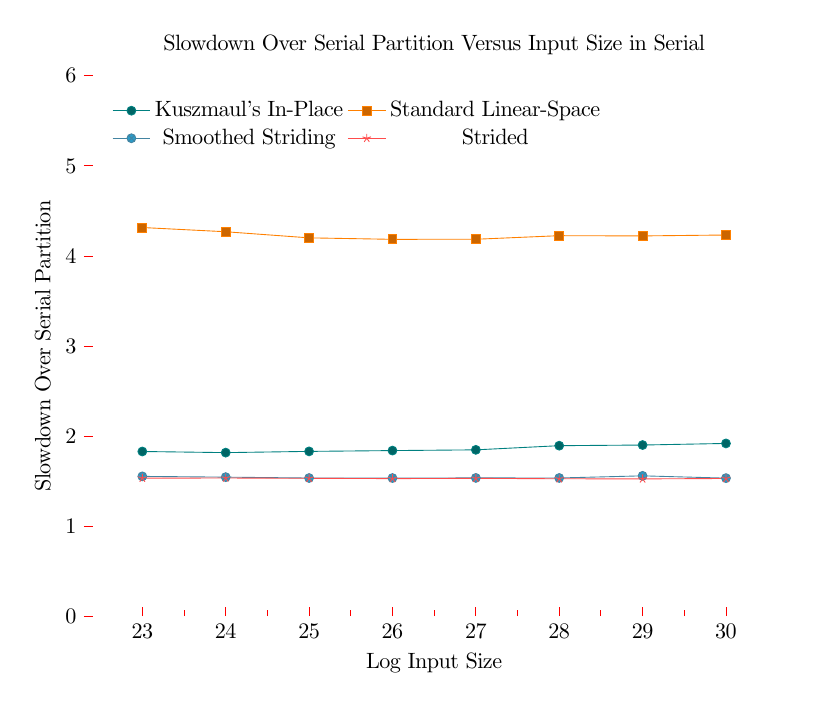
\begin{tikzpicture}[scale = .8]
\begin{axis}[
width = 5 in,
height = 4in,
title={Slowdown Over Serial Partition Versus Input Size in Serial},
xtick pos=left,
ytick pos=left,
ymax = 6,
ymin = 0,
legend style={draw=none},
axis line style = { draw = none },
legend pos= north west,
xtick = data,
xlabel={Log Input Size},
ylabel={Slowdown Over Serial Partition},
legend columns = 2,
scatter/classes=%
{a={mark=o,draw=blue}}]
%% Serial Baseline
%% baselines in ms: \addplot coordinates {( 23, 30.4 ) ( 24, 61 ) ( 25, 122.4 ) ( 26, 244.8 ) ( 27, 489.6 ) ( 28, 979.6 ) ( 29, 1963.4 ) ( 30, 3922.6 ) };
%% In-Place
\addplot coordinates {( 23, 1.82895) ( 24, 1.81639) ( 25, 1.83007) ( 26, 1.83905) ( 27, 1.84722) ( 28, 1.89343) ( 29, 1.90068) ( 30, 1.91837) };
%% In-Place Prefix-Sum
% \addplot coordinates {( 23, 2.75658) ( 24, 2.71803) ( 25, 2.68137) ( 26, 2.67157) ( 27, 2.67443) ( 28, 2.70131) ( 29, 2.70551) ( 30, 2.71713) };
%% Out-of-Place
\addplot coordinates {( 23, 4.31579) ( 24, 4.26885) ( 25, 4.20098) ( 26, 4.18464) ( 27, 4.18546) ( 28, 4.22519) ( 29, 4.22257) ( 30, 4.23265) };
%% %% High-Span
%% \addplot coordinates {( 23, 1.23684) ( 24, 1.23934) ( 25, 1.24346) ( 26, 1.24428) ( 27, 1.24632) ( 28, 1.24602) ( 29, 1.24417) ( 30, 1.2456) };
%% Cache-Friendly
\addplot coordinates {( 23, 1.55263) ( 24, 1.54426) ( 25, 1.53431) ( 26, 1.53431) ( 27, 1.53554) ( 28, 1.53491) ( 29, 1.55852) ( 30, 1.53317) };
%% Strided
\addplot coordinates {( 23, 1.53289) ( 24, 1.53443) ( 25, 1.53105) ( 26, 1.52778) ( 27, 1.53064) ( 28, 1.52613) ( 29, 1.5246) ( 30, 1.52919) };
\legend{Kuszmaul's In-Place, Standard Linear-Space, Smoothed Striding, Strided} % Low-Space, Med-Space, High-Space, Smoothed Striding, Strided
\end{axis}
\end{tikzpicture}
}
%% \def \serialnumtrials {5}
%% \def \serialblocksize {64}
%% \def \serialtable {
%% \begin{tikzpicture}[scale = .8]
%% \begin{axis}[
%% width = 5 in,
%% height = 4in,
%% title={Slowdown Versus Input Size in Serial},
%% xtick pos=left,
%% ytick pos=left,
%% ymax = 5,
%% ymin = 0,
%% legend style={draw=none},
%% axis line style = { draw = none },
%% legend pos= north west,
%% xtick = data,
%% xlabel={Log Input Size},
%% ylabel={Slowdown Over Serial Partition},
%% legend columns = 2,
%% scatter/classes=%
%% {a={mark=o,draw=blue}}]
%% %% Serial Baseline
%% %% baselines in ms: \addplot coordinates {( 23, 30.4 ) ( 24, 61 ) ( 25, 122.4 ) ( 26, 244.8 ) ( 27, 489.6 ) ( 28, 979.6 ) ( 29, 1963.4 ) ( 30, 3922.6 ) };
%% %% In-Place
%% \addplot coordinates {( 23, 1.82895) ( 24, 1.81639) ( 25, 1.83007) ( 26, 1.83905) ( 27, 1.84722) ( 28, 1.89343) ( 29, 1.90068) ( 30, 1.91837) };
%% %% In-Place Prefix-Sum
%% \addplot coordinates {( 23, 2.75658) ( 24, 2.71803) ( 25, 2.68137) ( 26, 2.67157) ( 27, 2.67443) ( 28, 2.70131) ( 29, 2.70551) ( 30, 2.71713) };
%% %% Out-of-Place
%% \addplot coordinates {( 23, 4.31579) ( 24, 4.26885) ( 25, 4.20098) ( 26, 4.18464) ( 27, 4.18546) ( 28, 4.22519) ( 29, 4.22257) ( 30, 4.23265) };
%% %% High-Span
%% \addplot coordinates {( 23, 1.23684) ( 24, 1.23934) ( 25, 1.24346) ( 26, 1.24428) ( 27, 1.24632) ( 28, 1.24602) ( 29, 1.24417) ( 30, 1.2456) };
%% %% Cache-Friendly
%% \addplot coordinates {( 23, 1.55263) ( 24, 1.54426) ( 25, 1.53431) ( 26, 1.53431) ( 27, 1.53554) ( 28, 1.53491) ( 29, 1.55852) ( 30, 1.53317) };
%% %% Strided
%% \addplot coordinates {( 23, 1.53289) ( 24, 1.53443) ( 25, 1.53105) ( 26, 1.52778) ( 27, 1.53064) ( 28, 1.52613) ( 29, 1.5246) ( 30, 1.52919) };
%% \legend{Low-Space, Med-Space, High-Space, Two-Layer, Cache-Friendly, Strided}
%% \end{axis}
%% \end{tikzpicture}
%% }
%% \def \serialnumtrials {1}
%% \def \serialblocksize {64}
%% \def \serialtable {
%% \begin{tikzpicture}[scale = .8]
%% \begin{axis}[
%% title={Slowdown Versus Input Size in Serial},
%% width = 5in, %%!!!!
%% height = 4in,
%% xtick pos=left,
%% ytick pos=left,
%% ymax = 5, %% !!!
%% ymin = 0,
%% legend style={draw=none},
%% axis line style = { draw = none },
%% legend pos= north west,
%% xtick = data,
%% xlabel={Log Input Size},
%% ylabel={Slowdown Over Serial Partition},
%% legend columns = 2,
%% scatter/classes=%
%% {a={mark=o,draw=blue}}]
%% %% Serial Baseline%% baselines in ms: \addplot coordinates {( 23, 30.4 ) ( 24, 60.8 ) ( 25, 121.4 ) ( 26, 243.8 ) ( 27, 487.4 ) ( 28, 975.8 ) ( 29, 1952.2 ) ( 30, 3902 ) };
%% %% In-Place
%% \addplot coordinates {( 23, 1.79605) ( 24, 1.82237) ( 25, 1.84185) ( 26, 1.84249) ( 27, 1.87033) ( 28, 1.90838) ( 29, 1.90687) ( 30, 1.91579) };
%% %% In-Place Prefix-Sum
%% \addplot coordinates {( 23, 2.58553) ( 24, 2.57237) ( 25, 2.57661) ( 26, 2.56932) ( 27, 2.56422) ( 28, 2.59459) ( 29, 2.60834) ( 30, 2.61107) };
%% %% Out-of-Place
%% \addplot coordinates {( 23, 3.98684) ( 24, 3.96711) ( 25, 3.96705) ( 26, 3.96308) ( 27, 3.98195) ( 28, 4.01537) ( 29, 4.03401) ( 30, 4.06079) };
%% %% High-Span
%% \addplot coordinates {( 23, 1.21053) ( 24, 1.23355) ( 25, 1.23558) ( 26, 1.23298) ( 27, 1.23677) ( 28, 1.24124) ( 29, 1.24096) ( 30, 1.23931) };
%% \legend{Low-Space, Med-Space, High-Space, Two-Layer} %% Two-layer instead of high-span everywhere
%% \end{axis}
%% \end{tikzpicture}
%% }
%% %% Speedup on 18 threads in table of size 268435456
%% \def \serialsortspeedup {0.780189}


\newcommand{\dec}{\operatorname{dec}}
\newcommand{\poly}{\operatorname{poly}}
\newcommand{\polylog}{\operatorname{polylog}}
\newcommand{\github}{\url{github.com/awestover/Parallel-Partition}}
\newcommand{\defn}[1]{{\textit{\textbf{\boldmath #1}}}}
\renewcommand{\paragraph}[1]{\vspace{0.09in}\noindent{\bf \boldmath #1.}} 
\usepackage{amsmath}
\usepackage{dsfont}
\def\E{\operatorname{\mathbb{E}}}
\usepackage{amssymb}
\usepackage{amsthm}
\usepackage{todonotes}
\usepackage{algorithm, algpseudocode}

\newtheorem{thm}{Theorem}[section]
\newtheorem{lem}[thm]{Lemma}
\newtheorem{prop}[thm]{Proposition}
\newtheorem{clm}[thm]{Claim}
\newtheorem{cor}[thm]{Corollary}
\newtheorem{conj}[thm]{Conjecture}
\theoremstyle{remark}
\newtheorem{rem}[thm]{Remark}
\newtheorem{ex}[thm]{Example}

\newtheorem{theorem}{Theorem}[section]
\newtheorem{definition}[thm]{Definition}
\newtheorem{lemma}[thm]{Lemma}
\newtheorem{proposition}[thm]{Proposition}
\newtheorem{claim}[thm]{Claim}
\newtheorem{corollary}[thm]{Corollary}
\newtheorem{conjecture}[thm]{Conjecture}
\theoremstyle{remark}
\newtheorem{remark}[thm]{Remark}
\newtheorem{example}[thm]{Example}
\newtheorem{observation}[thm]{Observation}

\usepackage{hyperref}

\usepackage{fancyhdr}
\pagestyle{fancy}
\fancyfoot[R]{\thepage}

\begin{document}

\title[]{Brief Announcement\\
In-Place Parallel-Partition Algorithms \\using Exclusive-Read-and-Write Memory}
\subtitle{An In-Place Algorithm With Provably Optimal Cache Behavior}

\author{William Kuszmaul}
\authornote{Supported by a Hertz Fellowship and a NSF GRFP Fellowship}
\affiliation{%
  \institution{Massachusetts Institute of Technology}
}
\email{kuszmaul@mit.edu}


\author{Alek Westover}
\authornote{Supported by MIT PRIMES.}
\email{alek.westover@gmail.com}


% The default list of authors is too long for headers.
\renewcommand{\shortauthors}{William Kuszmaul and Alek Westover}



%
% The code below should be generated by the tool at
% http://dl.acm.org/ccs.cfm
% Please copy and paste the code instead of the example below.
%
%% \begin{CCSXML}
%% <ccs2012>
%% <concept>
%% <concept_id>10003752.10003809.10010170.10010171</concept_id>
%% <concept_desc>Theory of computation~Shared memory algorithms</concept_desc>
%% <concept_significance>500</concept_significance>
%% </concept>
%% </ccs2012>
%% \end{CCSXML}

%% \ccsdesc[500]{Theory of computation~Shared memory algorithms}

%% \keywords{Parallel Partition, EREW PRAM, in-place algorithms}

\thispagestyle{fancy}
\begin{abstract}

We present an in-place algorithm for the parallel partition problem
that has linear work and polylogarithmic span. The algorithm uses only
exclusive read/write shared variables, and can be implemented using
parallel-for-loops without any additional concurrency considerations
(i.e., the algorithm is EREW). A key feature of the algorithm is that
it exhibits provably optimal cache behavior, up to small-order factors.

We also present a second in-place EREW algorithm that has linear work
and span $O(\log n \cdot \log \log n)$, which is within an
$O(\log\log n)$ factor of the optimal span. By using this low-span
algorithm as a subroutine within the cache-friendly algorithm, we are
able to obtain a single EREW algorithm that combines their theoretical
guarantees: the algorithm achieves span $O(\log n \cdot \log \log n)$ and
optimal cache behavior. As an immediate consequence, we also get an
in-place EREW quicksort algorithm with work $O(n \log n)$, span
$O(\log^2 n \cdot \log \log n)$.

Whereas the standard EREW algorithm for parallel partitioning is
memory-bandwidth bound on large numbers of cores, our cache-friendly
algorithm is able to achieve near-ideal scaling in practice by
avoiding the memory-bandwidth bottleneck. The algorithm's performance
is comparable to that of the Blocked Strided Algorithm of Francis,
Pannan, Frias, and Petit, which is the previous state-of-the art for
parallel EREW sorting algorithms, but which lacks theoretical
guarantees on its span and cache behavior.
\end{abstract}
\maketitle

\section{Introduction}

A \defn{parallel partition} operation rearranges the elements in an
array so that the elements satisfying a particular \defn{pivot
  property} appear first. In addition to playing a central role in
parallel quicksort, the parallel partition operation is used as a
primitive throughout parallel algorithms.\footnote{In several
  well-known textbooks and surveys on parallel algorithms
  \cite{AcarBl16,Blelloch96}, for example, parallel partitions are
  implicitly used extensively to perform what are referred to as
  \emph{filter} operations.}

A parallel algorithm can be measured by its \defn{work}, the time
needed to execute in serial, and its \defn{span}, the time to execute
on infinitely many processors. There is a well-known algorithm for
parallel partition on arrays of size $n$ with work $O(n)$ and span
$O(\log n)$ \cite{Blelloch96,AcarBl16}. Moreover, the algorithm uses
only exclusive read/write shared memory variables (i.e., it is an
\defn{EREW} algorithm).
The parallel-partition algorithm suffers from using a large amount of
auxiliary memory, however.
An algorithm's memory efficiency can be critical on large inputs.

\section{Preliminaries}\label{secprelim}

We begin by describing the parallelism and memory model used in
the paper, and by presenting background on the parallel partition problem.

\paragraph{Workflow Model} We consider a simple language-based model of parallelism in which algorithms achieve parallelism through the use of \defn{parallel-for-loops} (see, e.g.,
\cite{Blelloch96,AcarBl16,CLRS}); function calls within the inner loop
then allow for more complicated parallel structures (e.g., recursion). Our algorithms can also be implemented in the less restrictive PRAM model \cite{Blelloch96, AcarBl16}.

\paragraph{Memory Model}
Memory is \defn{exclusive-read} and \defn{exclusive-write} (i.e. we are in the
EREW model). That is, no two threads are ever permitted to attempt to read or
write to the same variable concurrently. Note that threads are not in lockstep
(i.e., they may progress at arbitrary different speeds), and thus the EREW
model requires algorithms to be data-race free in order to avoid the
possibility of non-exclusive data accesses.

In an \defn{in-place} algorithm, each thread is given $O(\polylog n)$
memory upon creation that is deallocated when the thread dies. This
memory can be shared with the thread's children. However, the depth of
the parent-child tree is not permitted to exceed $O(\polylog n)$.

\paragraph{Modeling Cache Misses}
We treat memory as consisting of fixed-size cache lines, each of some
size $b$. Each processor is assumed to have a small cache of
$\operatorname{polylog}{n}$ cache lines. A cache miss occurs on a
processor when the line being accessed is not currently in cache, in
which case some other line is evicted from cache to make room for the
new entry. Each cache is managed with a LRU (Least Recently Used)
eviction policy.

However, we may assume for the sake of analysis that each cache is managed by
the optimal off-line eviction strategy OPT (i.e. Furthest in the Future). This
is because, up to resource augmentation, LRU eviction is $(1 + 1/\polylog
n)$-competitive with OPT. Formally this is due to the following theorem by
Sleator and Tarjan:
\begin{theorem}[Resource Augmentation Theorem \cite{SleatorTa85}]
  LRU operating on a cache of size $K\cdot M$ for some $K>1$ will incur at most
  $1+\frac{1}{K-1}$ times the number of times cache misses of OPT operating on
  a cache of size $M$, for the same series of memory accesses.
  \label{thm:augmentation}
\end{theorem}
Because each processor's cache is managed by OPT (without loss of
generality), we can assume that each processor \defn{pins} certain
small arrays to cache (i.e., the elements of those arrays are never
evicted).


\paragraph{The (Standard) Linear-Space Parallel Partition} The linear-space
implementation of parallel partition consists of two phases
\cite{Blelloch96,AcarBl16}:

\noindent\emph{The Parallel-Prefix Phase: }In this phase, the algorithm first
creates an array $D$ whose $i$-th element $D[i] = \dec(A[i])$. Then the
algorithm constructs an array $S$ whose $i$-th element $S[i] = \sum_{j = 1}^i
D[i]$ is the number of predecessors in the first $i$ elements of $A$. The
transformation from $D$ to $S$ is called a \defn{parallel prefix sum} and can
be performed with $O(n)$ work and $O(\log n)$ span using a simple recursive
algorithm: (1) First construct an array $D'$ of size $n / 2$ with $D'[i] = D[2i
- 1] + D[2i]$; (2) Recursively construct a parallel prefix sum $S'$ of $D'$;
(3) Build $S$ by setting each $S[i] = S'[\lfloor i / 2 \rfloor] + A[i]$ for odd
$i$ and $S[i] = S'[i / 2]$ for even $i$. 

\noindent\emph{The Reordering Phase: }In this phase, the algorithm constructs
an output-array $C$ by placing each predecessor $A[i] \in A$ in position $S[i]$
of $C$. If there are $t$ predecessors in $A$, then the first $t$ elements of
$C$ will now contain those $t$ predecessors in the same order that they appear
in $A$. The algorithm then places each successor $A[i] \in A$ in position $t +
i - S[i]$. Since $i - S[i]$ is the number of successors in the first $i$
elements of $A$, this places the successors in $C$ in the same order that they
appear in $A$. Finally, the algorithm copies $C$ into $A$, completing the
parallel partition.

Both phases can be implemented with $O(n)$ work and $O(\log n)$
span. However, the algorithm uses multiple auxiliary arrays of size $n$.
Reducing the extra space below $o(n)$ has remained open until now, even when
the number of threads is fixed.


\section{An In-Place Algorithm \\with Span $O(\log n \log \log n)$}\label{sec:prefixbasedalg}
In this section, we present an overview of the key algorithmic ideas needed to
make the classic Parallel Partition algorithm in-place, with span $O(\log n \log\log n)$.
The algorithm we describe here is useful as a subroutine in our main algorithm,
the Smoothed Striding Algorithm, which is discussed in Section
\ref{sec:smoothing}.
The algorithm we discuss here has poor cache behavior, and so performs poorly
in practice. However, using it as a subroutine on a small subproblem in the
Smoothed Striding Algorithm will allow the Smoothed Striding Algorithm to
achieve span $O(\log n \log\log n)$ without sacrificing its cache behavior. 

\paragraph{Algorithm Outline}
Prior to beginning the algorithm, the first implicit step of the
algorithm is to count the number of predecessors in the array, in
order to determine whether the majority of elements are either
predecessors or successors. We assume without loss of generality that the total
number of successors in $A$ exceeds the number of predecessors, since otherwise
their roles can simply be swapped in the algorithm. Further, we assume for
simplicity that the elements of $A$ are distinct; this assumption is removed at
the end of Appendix \ref{secalg}.

Consider how to remove the auxiliary array $C$ from the Reordering
Phase. If one attempts to simply swap in parallel each predecessor
$A[i]$ with the element in position $j = S[i]$ of $A$, then the swaps
will almost certainly conflict. Indeed, $A[j]$ may also be a
predecessor that needs to be swapped with $A[S[j]]$. Continuing like
this, there may be an arbitrarily long list of dependencies on the
swaps.

To combat this, we begin the algorithm with a Preprocessing Phase in
which $A$ is rearranged so that every prefix is
\defn{successor-heavy}, meaning that for all $t$, the first $t$
elements contain at least $\frac{t}{4}$ successors. Then we compute
the prefix-sum array $S$, and begin the Reordering Phase. Using the
fact that the prefixes of $A$ are successor-heavy, the reordering can
now be performed in place as follows: (1) We begin by recursively
reordering the prefix $P$ of $A$ consisting of the first $4/5 \cdot n$
elements, so that the predecessors appear before the successors; (2)
Then we simply swap each predecessor $A[i]$ in the final $1/5 \cdot n$
elements with the corresponding element $S[A[i]]$. The fact that the
prefix $P$ is successor-heavy ensures that, after step (1), the final 
$\frac{1}{5} \cdot n$ elements of (the reordered) $P$ are successors. 
This implies in step (2) that for each of the swaps between predecessors $A[i]$
in the final $1/5 \cdot n$ elements and earlier positions $S[A[i]]$, the latter
element will be in the prefix $P$. In other words, the swaps are now conflict
free.

Next consider how to remove the array $S$ from the Parallel-Prefix
Phase. At face value, this would seem quite difficult since the
reordering phase relies heavily on $S$. Our solution is to
\emph{implicitly} store the value of every $O(\log n)$-th element of
$S$ in the ordering of the elements of $A$. That is, we break $A$ into
blocks of size $O(\log n)$, and use the order of the elements in each
block to encode an entry of $S$. (If the elements are not all
  distinct, then a slightly more sophisticated encoding is necessary.)
Moreover, we modify the algorithm for building $S$ to only construct
every $O(\log n)$-th element. The new parallel-prefix sum performs
$O(n / \log n)$ arithmetic operations on values that are implicitly
encoded in blocks; since each such operation requires $O(\log n)$
work, the total work remains linear.

Analysis of the algorithm yields the following theorem:
\begin{theorem}
  There exists an in-place algorithm using exclusive-read-write
  variables that performs parallel-partition with work $O(n)$ and span
  $O(\log n \cdot \log \log n)$.
\end{theorem}

\section{A Cache Efficient In-Place Parallel Partition}\label{sec:smoothing}

\paragraph{The Strided Algorithm \cite{FrancisPa92}}
The Smoothed Striding Algorithm borrows several structural ideas from a
previous algorithm of Francis and Pannan \cite{FrancisPa92}, which we call the
Strided Algorithm. The Strided Algorithm is designed to behave well on random
arrays $A$, achieving span $\tilde{O}(n^{2/3})$ and exhibiting only $n/b +
\tilde{O}(n^{2/3} / b)$  cache misses on such inputs. On worst-case inputs,
however, the Strided Algorithm has span $\Omega(n)$ and incurs $n/b +
\Omega(n/b)$ cache misses. Our algorithm, the Smoothed Striding Algorithm,
builds on the Strided Algorithm by randomly perturbing the internal structure
of the original algorithm; in doing so, we are able to provide provable
performance guarantees for arbitrary inputs, and to add a recursion step that
was previously impossible.

The original \defn{Strided Algorithm} consists of two steps: 
\begin{itemize}
\item \textbf{The Partial Partition Step.} Let $g \in \mathbb{N}$ be a
  parameter, and assume for simplicity that $gb \mid n$. Partition the
  array $A$ into $\frac{n}{gb}$ chunks $C_1, \ldots, C_{n / gb}$,
  each consisting of $g$ cache lines of size $b$.
  %% \footnote{In this
  %%   gection we zero-index arrays in order to enable modular arithmetic
  %%   on array indices.}
	For $i \in \{1, 2, \ldots, g\}$, define 
  $P_i$ to consist of the $i$-th cache line from each of the
  chunks $C_1, \ldots, C_{n / gb}$. One can think of the $P_i$'s
	as forming a strided partition of array $A$, since
  consecutive cache lines in $P_i$ are always separated by a fixed
  stride of $g - 1$ other cache lines.

  The first step of the algorithm is to perform an in-place serial
  partition on each of the $P_i$s, rearranging the elements within the
  $P_i$ so that the predecessors come first. This step requires work
  $\Theta(n)$ and span $\Theta(n/g)$.
\item \textbf{The Serial Cleanup Step. }For each $P_i$, define the
  \defn{splitting position} $v_i$ to be
  the position in $A$ of the first successor in (the already
  partitioned) $P_i$. Define $v_{\text{min}} = \min\{v_1, \ldots,
  v_{g}\}$ and define $v_{\text{max}} = \max\{v_1, \ldots, v_{g}\}$. Then the
  second step of the algorithm is to perform a serial partition on the
	sub-array \\$A[v_{\text{min}}],\ldots, A[v_{\text{max}}-1]$. This completes the   
    full partition of $A$.
\end{itemize}

Note that the Cleanup Step of the Strided Algorithm has no
parallelism, and thus has span $\Theta(v_{\text{max}} -
v_{\text{min}})$.  In general, this results in an algorithm with
linear-span (i.e., no parallelism guarantee).  When the number of
predecessors in each of the $P_i$'s is close to equal, however, the
quantity $v_{\text{max}} - v_{\text{min}}$ can be much smaller than
$\Theta(n)$. For example, if $b = 1$, and if each element of $A$ is
selected independently from some distribution, then one can use
Chernoff bounds to prove that with high probability in $n$,
$v_{\text{max}} - v_{\text{min}} \le O(\sqrt{n \cdot g \cdot \log
  n})$.  The full span of the algorithm is then $\tilde{O}(n/g +
\sqrt{n \cdot g})$, which optimizes at $g = n^{1/3}$ to
$\tilde{O}(n^{2/3})$. Since the Partial Partition Step incurs only $n
/ b$ cache misses, the full algorithm incurs $n + \tilde{O}(n^{2/3})$ cache
misses on a random array $A$.

Using Hoeffding's Inequality in place of Chernoff bounds, one can
obtain analogous bounds for larger values of $b$; in particular for $b
\in \operatorname{polylog}(n)$, the optimal span remains
$\tilde{O}(n^{2/3})$ and the number of cache misses becomes $n / b +
\tilde{O}(n^{2/3} / b)$ on an array $A$ consisting of randomly sampled
elements.\footnote{The original algorithm of Francis and Pannan
  \cite{FrancisPa92} does not consider the cache-line size $b$. Frias
  and Petit later introduced the parameter $b$ \cite{Frias08}, and
  showed that by setting $b$ appropriately, one obtains an algorithm
  whose empirical performance is close to the state-of-the-art.}


%% With this optimization, one advantage of the Strided Algorithm is that when $v_{\text{max}} - v_{\text{min}}$ is small, the total number of cache misses by the algorithm is close to the same as for a single scan through the data. 

\paragraph{The Smoothed Striding Algorithm}
To obtain an algorithm with provable guarantees for all inputs $A$, we
randomly perturb the internal structure of each of the $P_i$'s. Define
$U_1, \ldots, U_{g}$ (which play a role analogous to $P_1,
\ldots, P_g$ in the Strided Algorithm) so that each $U_i$ contains one
randomly selected cache line from each of $C_1, \ldots, C_{n /
  gb}$ (rather than containing the $i$-th cache line of each
$C_j$). This ensures that the number of predecessors in each $U_i$ is
a sum of independent random variables with values in $\{0, 1, \ldots,
n/g\}$.

By Hoeffding's Inequality, with high probability in $n$, the number of
predecessors in each $U_i$ is tightly concentrated around $\frac{\mu
  n}{g}$, where $\mu$ is the fraction of elements in $A$ that are
predecessors. It follows that, if we perform in-place partitions of
each $U_i$ in parallel, and then define $v_i$ to be the position in
$A$ of the first successor in (the already partitioned) $U_i$, then
the difference between $v_{\text{min}} = \min_i v_i$ and
$v_{\text{max}} = \max_i v_i$ will be small (regardless of the input array
$A$!).

Rather than partitioning $A[v_{\text{min}}],\ldots,
A[v_{\text{max}}-1]$ in serial, the Smoothed Striding Algorithm simply
recurses on the subarray. Such a recursion would not have been
productive for the original Strided Algorithm because the strided
partition $P_1', \ldots, P_g'$ used in the recursive subproblem would
satisfy $P_1' \subseteq P_1, \ldots, P_g' \subseteq P_g$ and thus each
$P_i'$ is already partitioned. That is, in the original Strided
Algorithm, the problem that we would recurse on is a worst-case input
for the algorithm in the sense that the partial partition step makes
no progress.


The main challenge in designing the Smoothed Striding Algorithm
becomes the construction of $U_1, \ldots, U_{g}$ without
violating the in-place nature of the algorithm. A natural approach
might be to store for each $U_i, C_j$ the index of the cache
line in $C_j$ that $U_i$ contains. This would require the storage of
$\Theta(n / b)$ numbers as metadata, however, preventing the algorithm
from being in-place. To save space, the key insight is to select a
random offset $X_j \in \{1, 2, \ldots, g\}$ within each $C_j$, and
then to assign the $(X_j + i \pmod g) + 1$-th cache line of $C_j$ to
$U_i$ for $i \in \{1, 2, \ldots, g\}$. This allows for us to construct
the $U_i$'s using only $O\left(\frac{n}{gb}\right)$ machine words
storing the metadata $X_1, \ldots, X_{n / gb}$. By setting $g$ to
be relatively large, so that $\frac{n}{gb} \le
\operatorname{polylog}(n)$, we can obtain an in-place algorithm that
incurs $n (1 + o(1))$ cache misses.

The recursive structure of the Smoothed Striding Algorithm allows for
the algorithm to achieve polylogarithmic span. As an alternative to
recursing, one can also use the in-place algorithm from the Appendix
 in order to partition \\ $A[v_{\text{min}}], \ldots,
  A[v_{\text{max}} - 1]$. This results in an improved span (since the
algorithm from the Appendix has span only \\ $O(\log n \log \log
n)$), while still incurring only $n (1 + o(1))$ cache misses (since
the cache-inefficient algorithm from the Appendix is only used
on a small subarray of $A$). We analyze both the recursive version of
the Smoothed Striding Algorithm, and the version which uses as a final
step the algorithm from the Appendix; one significant advantage
of the recursive version is that it is simple to implement in
practice.

\paragraph{Formal Algorithm Description} Let $b < n$ be the size of a cache line, let $A$ be an input array of size
$n$, and let $g$ be a parameter. (One should think of $g$ as being
relatively large, satisfying $\frac{n}{bg} \le
\operatorname{polylog}(n)$.)  We assume for simplicity that that $n$
is divisible by $gb$, and we define $s = \frac{n}{gb}$.
\footnote{This assumption can be made without loss of generality by treating $A$ as
an array of size $n' = n + {(gb - n \pmod {gb})}$, and then treating
the final $gb - n \pmod {gb}$ elements of the array as being
successors (which consequently the algorithm needs not explicitly
access). Note that the extra $n' - n$ elements are completely virtual, meaning they do not physically exist or reside in memory.
}

In the \defn{Partial Partition Step} the algorithm partitions the
cache lines of $A$ into $g$ sets $U_1, \ldots, U_{g}$ of size
$s = \frac{n}{gb}$ and then performs a serial partition on each $U_i$
in parallel over the $U_i$'s. To determine the sets
$U_1, \ldots, U_{g}$, the algorithm uses as metadata an array
$X = X[1], \ldots, X[s]$, where each $X[i] \in \{1, \ldots,
g\}$. 

Formally, the Partial Partition Step performs the following procedure:
\begin{itemize}
\item Set each of $X[1], \ldots, X[s]$ to be uniformly random and
  independently selected elements of $\{1, 2, \ldots, g\}$. For each $i \in
  \{1, 2, \ldots, g\}$, $j \in \{1, 2, \ldots, s\}$, define
  $$G_i(j) = (X[j] + i \pmod g) + (j - 1)g + 1.$$ Using this
  terminology, we define each $U_i$ for $i \in \{1, \ldots, g\}$ to
  contain the $G_i(j)$-th cache line of $A$ for each $j \in \{1, 2,
  \ldots, s\}$. That is, $G_i(j)$ denotes the index of the $j$-th
  cache line from array $A$ contained in $U_i$.

  Note that, to compute the index of the $j$-th cache line in $U_i$,
  one needs only the value of $X[j]$. Thus the only metadata needed by
  the algorithm to determine $U_1, \ldots, U_g$ is the array
  $X$. If $|X| = s = \frac{n}{gb} \le \operatorname{polylog}(n)$, then
  the algorithm is in place.
  
\item The algorithm performs an in-place (serial) partition on each
  $U_i$ (and performs these partitions in parallel with one
  another). In doing so, the algorithm, also collects
  $v_{\text{min}}=\min_i{v_i}$, $v_{\text{max}}=\max_i{v_i}$, where
	each $v_i$ with $i \in \{1, \ldots, g\}$ is defined to be the index
  of the first successor in $A$ (or $n$ if no such successor
  exists).\footnote{One can calculate $v_{\text{min}}$ and
    $v_{\text{max}}$ without explicitly storing each of $v_1, \ldots,
		v_{g}$ as follows. Rather than using a standard $g$-way parallel
		for-loop to partition each of $U_1, \ldots, U_{g}$, one can
    manually implement the parallel for-loop using a recursive
    divide-and-conquer approach. Each recursive call in the
    divide-and-conquer can then simply collect the maximum and minimum
    $v_i$ for the $U_i$'s that are partitioned within that recursive
    call. This adds $O(\log n)$ to the total span of the Partial
    Partition Step, which does not affect the overall span
    asymptotically. %% In practice, this can also be implemented using
    %% CilkPlus Reducers (or OpenMP Reductions) \cite{FrigoLe09}, though
    %% empirically we have found explicitly implementing the
    %% divide-and-conquer structure to be worthwhile for performance.
  }
  
  The array $A$ is now partially partitioned, i.e. $A[i]$ is a
  predecessor for all $i \le v_{\text{min}}$, and $A[i]$ is a successor
  for all $i > v_{\text{max}}$.
\end{itemize}

The second step of the Smoothed Striding Algorithm is to complete the
partitioning of $A[v_{\text{min}} + 1], \ldots, A[v_{\text{max}}]$. This can be done
in one of two ways: The \defn{Recursive Smoothed Striding Algorithm}
partitions $A[v_{\text{min}} + 1], \ldots, A[v_{\text{max}}]$ recursively using the
same algorithm (and resorts to a serial base case when the subproblem
is small enough that $g \le O(1)$); the \defn{Hybrid Smoothed Striding
  Algorithm} partitions $A[v_{\text{min}} + 1], \ldots, A[v_{\text{max}}]$ using the
in-place algorithm given in Theorem \ref{thminplace} with span $O(\log
n \log \log n)$. In general, the Hybrid algorithm yields better
theoretical guarantees on span than the recursive version; on the
other hand, the recursive version has the advantage that it is
simple to implement as fully in-place, and still achieves
polylogarithmic span. 

% Detailed pseudocode for the Recursive Smoothed Striding Algorithm can
% be found in Appendix \ref{sec:pseudocode}.

%% note: g > s should hold
\paragraph{Algorithm Analysis} 
We prove the following proposition regarding the Partial Partition Step of the
Smoothed Striding Algorithm.
\begin{proposition}
  \label{prop:generalResult}
  Let $\epsilon \in (0, 1/2)$ and $\delta \in (0, 1/2)$ such that
  $\epsilon \ge \frac{1}{\poly(n)}$ and $\delta \ge
  \frac{1}{\polylog(n)}$. Suppose $s > \frac{\ln
    (n/\epsilon)}{\delta^2}$. Finally, suppose that each processor has
  a cache of size at least $s + c$ for a sufficiently large constant
  $c$.

  Then the Partial-Partition Algorithm achieves work $O(n)$; achieves
  span $O\paren*{b \cdot s}$; incurs $\frac{s+n}{b} + O(1)$ cache
  misses; and guarantees with probability $1 - \epsilon$ that
  $$v_{\text{max}}-v_{\text{min}} < 4 n \delta.$$
\end{proposition}

Using this we can analyze the hybrid and recursive smoothed striding algorithms.

We will assume that both the hybrid and the recursive algorithms use $\epsilon
= 1/n^c$ for $c$ of our choice (i.e. with high probability in $n$). Moreover,
the Recursive Smoothed Striding Algorithm continues to use the same value of
$\epsilon$ within recursive subproblems (i.e., the $\epsilon$ is chosen based
on the size of the first subproblem in the recursion), so that the entire
algorithm succeeds with high probability in $n$.

For both algorithms, the choice of $\delta$ results in a tradeoff between cache
misses and span. For the Recursive algorithm, we allow for $\delta$ to be
chosen arbitrarily at the top level of recursion, and then fix $\delta  =
\Theta(1)$ to be a sufficiently small constant at all levels of recursion after
the first; this guarantees that we at least halve the size of the problem
between recursive iterations\footnote{In general, setting $\delta = 1/8$ will
result in the problem size being halved. However, this relies on the assumption
that $gb \mid n$, which is only without loss of generality by allowing for the
size of subproblems to be sometimes artificially increased by a small amount
(i.e., a factor of $1 + gb / n = 1 + 1/s$). One can handle this issue by
decreasing $\delta$ to, say, $1/16$.}. Optimizing $\delta$ further (after the
first level of recursion) would only affect the number of undesired cache
misses by a constant factor.

Formally we prove the following performance results for these algorithms:
\begin{corollary}
	\label{cor:fullPartition}
Suppose $b \le o(\log \log n)$. Then the Hybrid Smoothed Striding Algorithm using $\delta = \Theta\big(\sqrt{b/\log\log n}\big)$, achieves work $O(n)$, and with high probability in $n$, achieves span $O(\log n \log\log n)$ and incurs fewer than $(n+o(n))/b$ cache misses.\\\\
\end{corollary}

\begin{corollary}
  \label{cor:groupedPartitionAlg}
	With high probability in $n$, the Recursive Smoothed Striding Algorithm using parameter $\delta=1/\sqrt{\log n}$:
  achieves work $O(n)$, attains span $O(b\log^2 n)$, and incurs $n/b \cdot (1 + O(1 / \sqrt{\log n}))$ cache misses. 
\end{corollary}

\section{Performance Comparisons}\label{secexp}
\begin{figure}[h]
  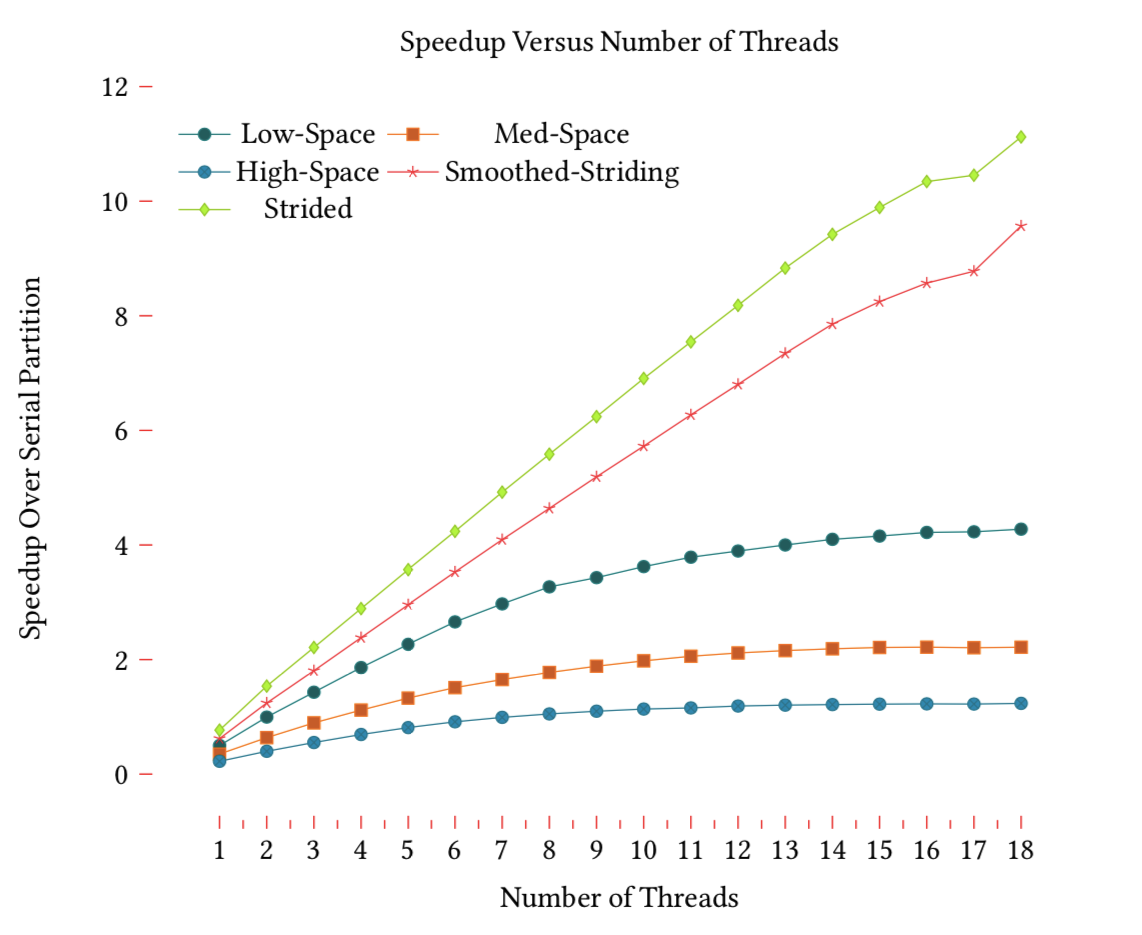
\includegraphics[width=\linewidth]{graph_performance.png}
% \CILKtable 
% \caption{We compare the performance of various partition implementations, relative to the Libc serial baseline, on random arrays of size $2^{30}$.
%  The $x$-axis plots the number of worker threads being used, and the $y$-axis
%  plots the multiplicative speedup over the serial baseline. Each time
%  (including the serial baseline) is averaged over five trials.}
%  \label{tablecilk}
\end{figure}

\bibliographystyle{ACM-Reference-Format}
\bibliography{paper}

\end{document}
